\documentclass[12pt]{article}
\usepackage{geometry}
 \geometry{
 a4paper,
 total={170mm,257mm},
 left=20mm,
 top=20mm,
 }

\usepackage{hyperref}
\usepackage{graphicx}
\usepackage{subcaption}
\usepackage{xcolor}
\usepackage[backend=biber, style=ieee]{biblatex}

\usepackage{mathtools}

\usepackage{acronym}

\usepackage{glossaries}

\usepackage[nameinlink,noabbrev]{cleveref} % nice for referencing

\crefname{equation}{equation}{equations}
\Crefname{equation}{Equation}{Equations}
\crefname{table}{table}{tables}
\Crefname{table}{Table}{Tables}
\crefname{figure}{fig.}{figures}
\Crefname{figure}{Fig.}{Figures}

\title{Tittel}
\author{Forfatter}
\date{}

\addbibresource{bibliography.bib}



\newacronym{ffnn}{FFNN}{Fast-forward neural network}    % Feed-Forward?
\newacronym{ann}{ANN}{Artificial neural network}
\newacronym{rnn}{RNN}{Recurrent neural network}
\newacronym{lstm}{LSTM}{Long short-term memory}
\newacronym{llm}{LLM}{Large language models}
\newacronym{bptt}{BPTT}{Backpropagation through time}
\newacronym{nlp}{NLP}{Natural language processing}

\newacronym{gpu}{GPU}{General processing unit}
\newacronym{tpu}{TPU}{Tensor processing unit}

\newacronym{relu}{ReLU}{Rectified linear unit}


% % \usepackage{acronym}
\acrodef{rnn}[RNN]{Recurrent Neural Network}
\acrodef{ffnn}[FFNN]{Feed-Forward Neural Network}
\acrodef{mlp}[MLP]{Multi-Layer Perceptron}
    % Acronyms defined by acronym environment



\begin{document}

\maketitle

\section{Abstract}

With the rapid development of and easy access to many different machine learning tools and programming libraries, it is easy to forget the building stones of what makes machine learning and neural networks what they are today, and what got them here. To try and oppose this effect we will in this paper take apart a classical machine learning model and through only the use of Python and basic libraries such as Numpy, build a \gls{rnn} piece by piece, from the forward pass down to each derivative in the \gls{bptt} algorithm to get the fundamental understanding of this historical machine learning model and see whether its performance can meet our expectations.

\section{Curtain-raiser}

Machine learning is becoming a more prominent part of data processing and society day by day, and thus several different approaches to machine learning have emerged as time has passed, such as supervised, unsupervised, and reinforcement learning. The first two of these approaches have seen the most success through the use of \gls{ffnn}s with backpropagation, which is versatile and greatly scalable. One downside of these conventional neural networks is their limitation concerning processing sequential data, there is no correlation between time-dependent data, or data samples passed into the network. There is a correlation between data points passed into the network at the same time, however, if the length of the data to be passed into the network changes, the whole network will have to be initialised again. As a resolution to this problem, artificial neural networks designed for the processing of sequential data have been developed, examples of this are \gls{rnn}s, \gls{lstm}, and Transformers, where the latter have had a substantial role in the rapid improvements of \gls{llm} in recent times. The \gls{rnn} is the predecessor of both the \gls{lstm} and the transformer architectures, and it is what we will focus on in this paper. We will focus on the \gls{rnn} architecture because when working with machine learning today there are so many tools available making the process of getting all kinds of neural networks up and running in no time. However, despite enabling developers to develop and deploy products and services at higher rates than previously possible, it also omits the need for the developers to have a deep understanding of what they're working with. That is what we're aiming at in this paper, we aim to develop a thorough understanding of the \gls{rnn} architecture by implementing it from scratch in Python only with Numpy \cite{Numpy} and some supplementary libraries, without the use of any available machine learning tools.


\section{Background}
\subsection{Sequential data}    \label{sec:seq-data}
Sequential data is any data that comes in a sequence. That is any set of data where the data points have a dependency on the previous data points. Many types of data can be defined as sequential. These include, but are not limited to: \cite{jamesDeepLearning2023}
\begin{description}
    \item[Documents.] Different types of documents are sequential in nature. This is easy to understand when you consider how the order in which words are written affect the meaning of the text in it.
    \item[Measurements in time series.] There are several types of measurement where earlier measurements tell us something about what will or might happen. For example are weather patterns well described as a sequence, since shifts in weather happen gradually, and not fully at random.
    \item[Financial time series.] Stock processes and stock market indices are examples of financial time series where each value is dependent on previous values.
    \item[Sound recordings.] Speech, music, and other sound recordings are generally sequential in that if you were to sample them at random positions and play the resulting recording, they would not make sense at all. Sound recordings are sequential in much the same way as text documents.
    % \item[Handwriting]      % Not sure how to explain the sequentiality of handwriting.
\end{description}

\noindent
As we can see, there are many applicable data sets that can best be described as a sequence.

\subsubsection{Prediction of sequential data}
Of course, we could take sequential data sets and feed them into a \gls{ffnn}, however, this does not take into consideration the correlation between data points in order. This is what \gls{rnn}s are good at, but we will get back to that in \cref{sec:rnn}.

\subsection{Recurrent Neural Networks}  \label{sec:rnn}
The origin of \gls{rnn} can be said to stem back to the Ising machine in 1925, however, it did not learn, and it was first made adaptive in 1972 by Shun'ichi Amari. In 1982 the Hopfield network was described through the Ising memory model by Amari, and in 1986 the recurrent neural network as we know it today was proposed by David Rumelhart with the emergence of backpropagation \cite{rumelhart_learning_1986}. The appeal of an \gls{rnn} is as mentioned in the introduction the processing of sequential data or time sequences, and the ability to process sequences of different lengths in the same network. 

The \gls{rnn} is an extension of the \gls{mlp}, also known as a \gls{ffnn}. 
% We have already described \gls{ffnn}s in \cref{sec:ffnn}.
What distinguishes an \gls{rnn} from an \gls{ffnn} is that \gls{rnn}s take sequential data as input (see section \cref{sec:seq-dat}). \cite{schmidtRecurrentNeuralNetworks2019} Actually, \gls{ffnn}s can take the same data as input, but it won't take their sequential nature into consideration in the way that an \gls{rnn} will. This is because an \gls{rnn} takes all previous timesteps into consideration.

\begin{figure}
  % \centering
  \begin{subfigure}{0.45\columnwidth}
    \centering
    \begin{adjustbox}
      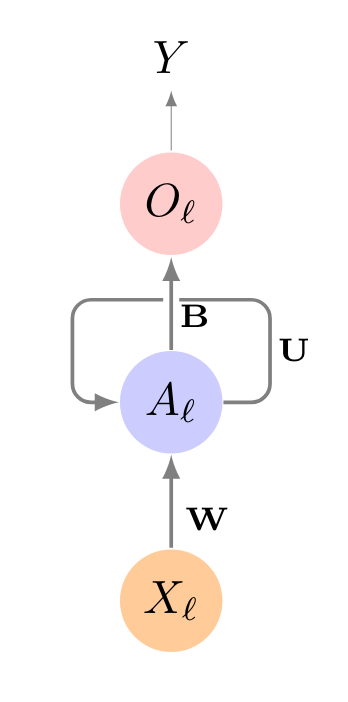
\includegraphics[height=5cm]{texfiles/figures/rnn-folded.png}
    \end{adjustbox}
    \caption{Folded RNN architecture}
    \label{}
  \end{subfigure}
  % \hfill
  \begin{subfigure}{0.45\columnwidth}
    \centering
    \begin{adjustbox}
      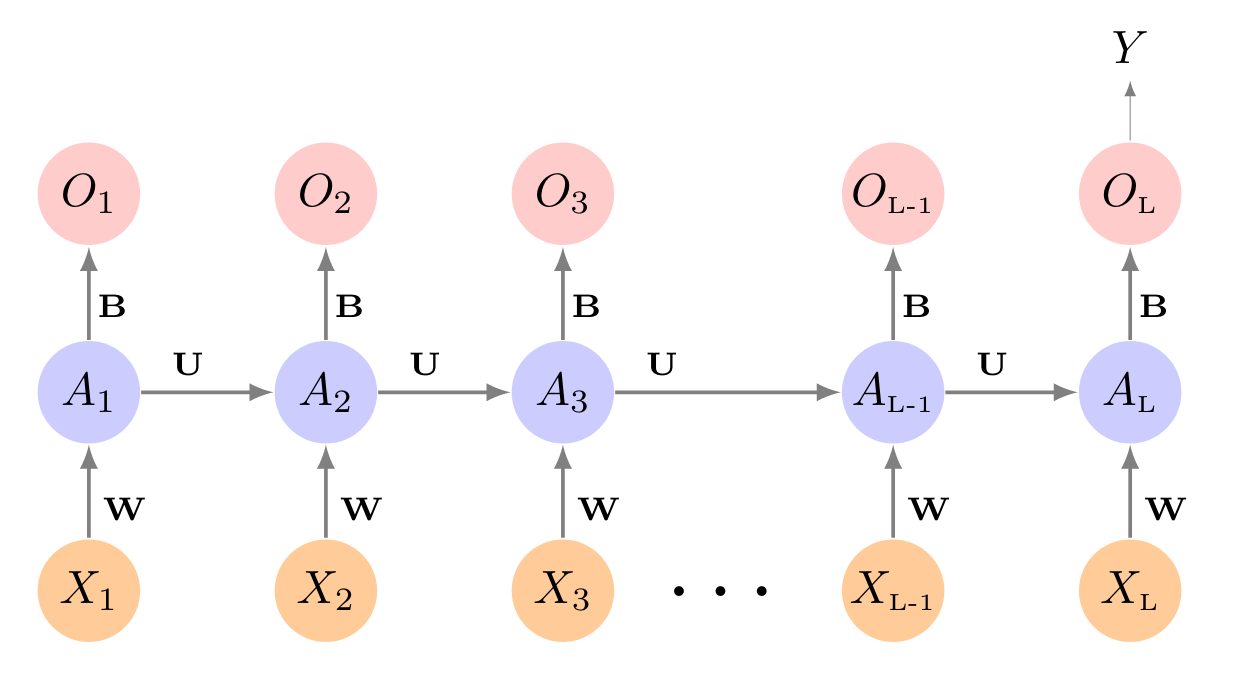
\includegraphics[height=5cm]{texfiles/figures/rnn-unfolded.png}
    \end{adjustbox}
    \caption{Unfolded RNN architecture}
    \label{fig:rnn-unfolded}
  \end{subfigure}
  \caption{RNN architecture \cite{james_deep_2023}}
  \label{fig:rnn-arch}
\end{figure}

\cref{fig:rnn-folded} shows the architecture of aN \gls{rnn}. 


\section{Method}
Since the purpose of this project is to investigate the math and implementations underlying a recurrent neural network (\gls{rnn}), the \gls{rnn} architecture and its surroundings - such as optimisation algorithms and data processing - are implmented totally without traditional machine learning (ML) libraries like Torch and Scikit-learn. All code is written in Python, using numpy \cite{harrisArrayProgrammingNumPy2020} for all numerical processing, such as vector and matrix multiplication. The \gls{rnn} is implemented in its most basic form, often denoted as a \textit{vanilla \gls{rnn}}. Nevertheless, the implementation handles a wide variety of data types and allows for configurability of optimisation algorithms and activation functions. The focus of the implementation has been natural language data. However, the model could also be used for other time series data, such as learning to predict interest rates, or mimic and generate oscillations like sine waves. None of the implementations exploits \gls{gpu}s or \gls{tpu}s, which has been found to increase FLOPS for some \gls{rnn} models \cite{wang_benchmarking_2019}. The implementation could therefore be slower than its \gls{gpu} or \gls{tpu} optimised versions, but this is not always the case with \gls{rnn}s, as all data must be processed sequentially - at least for our vanilla \gls{rnn} implementation. Below is a description of the code experiments.

\subsection{Python implementation}

\subsubsection*{Model architecture}
The \gls{rnn} is built as a class, where all nodes and layers are built simply by initialising matrices of dimensions corresponding to the layers. The number of input nodes $N$ is automatically determined based on the length of each data sample, which corresponds to the number of features if thinking in terms of \gls{ffnn}s. The number of hidden nodes $M$ is determined by the user. The number of output nodes $K$ is determined by the dimension of the target vector. This means that the input to hidden weights $\mathbf{U}$, the hidden to hidden (recurrent) weights $\mathbf{W}$ and the hidden to output weights $\mathbf{V}$ has the dimensions
\begin{align*}
    dim(\mathbf{U}) &= M \times N \\
    dim(\mathbf{W}) &= M \times M \\
    dim(\mathbf{V}) &= K \times M
\end{align*}
Adding bias terms on the hidden layer $\mathbf{b}$ and on the output layer $\mathbf{c}$
\begin{align*}
    dim(\mathbf{b}) &= 1 \times M  \\
    dim(\mathbf{c}) &= 1 \times K
\end{align*}

\subsubsection*{Going forwards}
All data samples share the above mentioned parameters $\mathbf{U, W, b, V, c}$. A forward pass of one data sample can be described by the following equations:
\begin{align}
    \mathbf{a}^{(t)} &= \mathbf{b + Wh^{(t-1)} + Ux^{(t)}} \\
    \mathbf{h}^{(t)} &= activation(\mathbf{a}^{(t)})\\
    \mathbf{o}^{(t)} &= \mathbf{c + Vh}^{(t)} \\
    \mathbf{\hat{y}}^{(t)} &= postprocessing(\mathbf{o}^{(t)})
\end{align}
The activation function employed in the experiments is the hyperbolic tangent function
\begin{equation}
    \g(z) = \tanh(z)
\end{equation}
function. This function is closely related to the sigmoid activation function, but resembles the identity function more than the sigmoid, as $\tanh(0) = 0$, while $\sigma(0) &= \frac12$. The trait of resembling the identity function makes optimisation easier, because optimising the network resembles optimising a linear model, according to Goodfellow et al., 2016 \cite{goodfellow_deep_2016}. The \gls{relu}, identity and sigmoid activation functions are also included in the code for completeness.
The postprocessing stage, which could also be described as an activation function on the output layer, is either the Softmax function
\begin{equation}
    g(z) = \frac{\exp(z)}{\sum \exp(z)},
\end{equation} 
when doing classification, or the identity function,
\begin{equation}
    g(z) = z,
\end{equation}
when doing regression. \\

\subsubsection*{Going backwards}
\color{red}Denne er ganske uferdig - må lese litt mer\color{black}
% The choice of loss-function and choice of output activation are tightly coupled. Since all differentiation 
Our experiments can be divided into two: estimating which class should be the next based on previous seen labels, and which number/vector should be the next based on previous labels. 
For the classification case, the goal is to ??maximize the probability of the observed data?? by estimating parameters (here: $\mathbf{U, V, W, b, c}$). The estimated parameters yielding the highest maximum likelihood are called the maximum likelihood estimates. These parameters can be estimated by minimizing the cross-entropy between the model distribution and the data. %To ease calculations, and because of the concavity of the problem, we derive the following cost-function:
This cross-entropy function, which is a function of inputs at time t ($\mathbf{x^{(t}}$) and outputs ($\mathbf{y^{(t}}$):
\begin{align}
    &C\left(\{\mathbf{x}^{(1)},...,\mathbf{x}^{(\tau)}\}, \{\mathbf{y}^{(1)},...,\mathbf{y}^{(\tau)}\}\right) \\
    &= \sum_t C^{(t)}
    \shortintertext{Can be written as (note: $y^{(t)}$ is an entry in the output vector $\mathbf{y}^{(t)}$):}
    &= -\sum_t log\;p\left(y^{(t)}|\{\mathbf{x}^{(1)},...,\mathbf{x}^{(t)}\}\right)
\end{align}

The cost function is the negative likelihood function. Minimizing this function is the same as maximizing the likelihood of the parameters. 

For the regression case, where estimating numerical values, the 
% After forward passing data, the model must learn from mistakes by updating the weights. This is done through stochastic gradient descent, where the gradient calculation is done by an algorithm called Back Propagation Through Time (BPTT) \cite{goodfellow_deep_2016}. This algorithm resembles the common deep learning optimisation strategy Back Propagation
Below we derive the gradients of the nodes in the computational graph from the deep learning book. These gradients must propagate backward through time, from time $t=\tau$ down to $t=0$.
\par
The gradient of the cost function at the output, $\mathbf{o}$, at time \textit{t} is
\begin{align}
    \nabla_{\mathbf{o}^{(t)}} C &= \frac{\delta C}{\delta o^{(t)}}
    = \frac{\delta C}{\delta C^{(t)}}\frac{\delta C^{(t)}}{\delta o^{(t)}}
    = \hat{y}^{(t)} - \mathbf{1}_{i=y^{(t)}}
    % \text{i is indices in $\hat{y}^{(t)}$. The predicate at the end of the previous line makes sense if one considers for example the $\hat{y}^{(t)}$ consisting of probabilities for all the different characters.}
\end{align}

We have found a general expression for the gradient at the $\mathbf{o}^{(t)}$-nodes. The next step is to find an expression for the gradient of the final hidden (computational) node, at time $\tau$: $\mathbf{h}^{(\tau)}$. Its only descendant is $\mathbf{o}^{(\tau)}$, which means its gradient is solely dependent on this node, which makes it a good starting point for the later gradient calculations.

\begin{align}
    \nabla_{\mathbf{h}^{(\tau)}} C &= \left(\nabla_{\mathbf{o}^{(\tau)}}C\right) \frac{\delta \mathbf{o}^{(\tau)}}{\delta \mathbf{h}^{(\tau)}}\\
    &= \left(\nabla_{\mathbf{o}^{(\tau)}}C\right) \mathbf{V}\\
    \nabla_{\mathbf{h}^{(\tau)}} C &= \mathbf{V}^{\top} \left(\nabla_{\mathbf{o}^{(\tau)}}C\right)
    % \nabla_{\mathbf{h}{(\tau)}} C &= \mathbf{V}^{\top}\left(\hat{y}^{(\tau)} - \mathbf{1}_{i=y^{(\tau)}}\right) \\
\end{align}
Where all the right-hand side terms are known from before. \par

The only nodes that need gradient computation now, are all the hidden states preceding the last. I.e., for $\mathbf{h}^{(t)}$, where $t = \{0,...,\tau-1\}$. For these time steps, the gradient is influenced by both the gradient at $\mathbf{o}^{(t)}$, as well as all the preceding hidden state gradients. Remember that the preceding hidden state of $\mathbf{h}^{(t)}$ is $\mathbf{h}^{(t+1)}$, which has preceding hidden state $\mathbf{h}^{(t+2)}$, and so on. We are calculating the gradient starting from $t=\tau-1$, working our way down to $t=0$: \par
% \begin{align}
%     \shortintertext{Denne linja kan være veldig feil}
%     \nabla_{\mathbf{h}^{(t-1)}} C &= \nabla_{\mathbf{h}^{(t)}} C + \nabla_{\mathbf{o}^{(t-1)}}C \\ 
%     \nabla_{\mathbf{h}^{(t-1)}} C &= \nabla_{\mathbf{h}^{(t)}} C \frac{\delta}{\delta} + V^{\top}\left(\nabla_{\mathbf{o}^{(t-1)}}C\right)
% \end{align}

\begin{align}
    \nabla_{\mathbf{h}^{(\tau-1)}} C &= \color{blue}\nabla_{\mathbf{o}^{(\tau-1)}}C \frac{\delta \mathbf{o}^{(\tau-1)}}{\delta \mathbf{h}^{(\tau-1)}} + \nabla_{\mathbf{h}^{(\tau)}}C \frac{\delta \mathbf{h}^{(\tau)}}{\delta \mathbf{h}^{(\tau-1)}} \\
    \nabla_{\mathbf{h}^{(\tau-2)}} C &= \color{red}\nabla_{\mathbf{o}^{(\tau-2)}}C \frac{\delta \mathbf{o}^{(\tau-2)}}{\delta \mathbf{h}^{(\tau-2)}} + \color{blue}\nabla_{\mathbf{h}^{(\tau-1)}}C \color{red} \frac{\delta \mathbf{h}^{(\tau-1)}}{\delta \mathbf{h}^{(\tau-2)}} \\
    \nabla_{\mathbf{h}^{(\tau-3)}} C &= \nabla_{\mathbf{o}^{(\tau-3)}}C \frac{\delta \mathbf{o}^{(\tau-3)}}{\delta \mathbf{h}^{(\tau-3)}} + \color{red}\nabla_{\mathbf{h}^{(\tau-2)}}C \color{black} \frac{\delta \mathbf{h}^{(\tau-2)}}{\delta \mathbf{h}^{(\tau-3)}} \\
    &= \nabla_{\mathbf{o}^{(\tau-3)}}C \frac{\delta \mathbf{o}^{(\tau-3)}}{\delta \mathbf{h}^{(\tau-3)}} + \color{red}\left(\nabla_{\mathbf{o}^{(\tau-2)}}C \frac{\delta \mathbf{o}^{(\tau-2)}}{\delta \mathbf{h}^{(\tau-2)}} + \color{blue}\nabla_{\mathbf{h}^{(\tau-1)}}C\color{red} \frac{\delta \mathbf{h}^{(\tau-1)}}{\delta \mathbf{h}^{(\tau-2)}} \right) \color{black} \frac{\delta \mathbf{h}^{(\tau-2)}}{\delta \mathbf{h}^{(\tau-3)}} \\
    &= \nabla_{\mathbf{o}^{(\tau-3)}}C \frac{\delta \mathbf{o}^{(\tau-3)}}{\delta \mathbf{h}^{(\tau-3)}} + \color{red}\left(\nabla_{\mathbf{o}^{(\tau-2)}}C \frac{\delta \mathbf{o}^{(\tau-2)}}{\delta \mathbf{h}^{(\tau-2)}} + \color{blue}\left(\color{blue}\nabla_{\mathbf{o}^{(\tau-1)}}C \frac{\delta \mathbf{o}^{(\tau-1)}}{\delta \mathbf{h}^{(\tau-1)}} + \nabla_{\mathbf{h}^{(\tau)}}C \frac{\delta \mathbf{h}^{(\tau)}}{\delta \mathbf{h}^{(\tau-1)}} \right)\color{red} \frac{\delta \mathbf{h}^{(\tau-1)}}{\delta \mathbf{h}^{(\tau-2)}} \right) \color{black} \frac{\delta \mathbf{h}^{(\tau-2)}}{\delta \mathbf{h}^{(\tau-3)}} \\
    \shortintertext{Generally:}
    \nabla_{\mathbf{h}^{(t)}} C &= \nabla_{\mathbf{o}^{(t)}}C \frac{\delta \mathbf{o}^{(t)}}{\delta \mathbf{h}^{(t)}} + \nabla_{\mathbf{h}^{(t+1)}}C \frac{\delta \mathbf{h}^{(t+1)}}{\delta \mathbf{h}^{(t)}}
    % &= \nabla_{\mathbf{o}^{(\tau-2)}}C \frac{\delta \mathbf{o}^{(\tau-2)}}{\delta \mathbf{h}^{(\tau-2)}} + \color{blue}\left(\nabla_{\mathbf{o}^{(\tau-1)}}C \frac{\delta \mathbf{o}^{(\tau-1)}}{\delta \mathbf{h}^{(\tau-1)}} + \nabla_{\mathbf{h}^{(\tau)}}C \frac{\delta \mathbf{h}^{(\tau)}}{\delta \mathbf{h}^{(\tau-1)}}\right)\color{black}\frac{\delta \mathbf{h}^{(\tau-1)}}{\delta \mathbf{h}^{(\tau-2)}}
    % \nabla_{\mathbf{h}^{(0)}} C &= \nabla_{\mathbf{o}^{(0)}}C + \nabla_{\mathbf{h}^{(\tau-3)}}C \\
\end{align}\par
Some parts of the equations above have been colored to emphasize the parts that we take with us from one gradient calculation to the next. \par
It is observable that the gradient at time $t$ is indeed dependent on all later time steps $t + 1, t + 2, t + n$, as well as the current output. The influence from current output can be seen before the first (+), while the influence from previous states can be observed after the first (+). \par

The final step is to calculate the gradient of the parameter nodes $\mathbf{U, W, b, V, c}$. To find these gradients, we must differentiate $\mathbf{h}^{(t)}$. Calculating the derivative of $\mathbf{h}^{(t)}$ involves differentiating the activation function using the chain rule. In the equations below, the chain rule is applied to differentiate the activations with respect to different parameters, but the activation function itself is not differentiated because it depends on which activation function is in use. It is instead denoted as $\nabla_{activation}$.
\begin{align*}
    \nabla_\mathbf{c}C &= \sum_t \left(\nabla_{\mathbf{o}^{(t)}}C\right) \frac{\delta \mathbf{o}^{(t)}}{\delta \mathbf{c}^{(t)}} &&= \sum_t \left(\nabla_{\mathbf{o}^{(t)}}C\right) \cdot 1 \\
    \nabla_\mathbf{V}C &= \sum_t \left(\nabla_{\mathbf{o}^{(t)}}C\right) \frac{\delta \mathbf{o}^{(t)}}{\delta \mathbf{h}^{(t)}} &&= \sum_t \left(\nabla_{\mathbf{o}^{(t)}}C\right)\mathbf{h^{(t)}} \\
    \nabla_\mathbf{b}C &= \sum_t \left(\nabla_{\mathbf{h}^{(t)}}C\right) \frac{\delta \mathbf{h}^{(t)}}{\delta \mathbf{b}^{(t)}} &&= \sum_t \left(\nabla_{\mathbf{h}^{(t)}}C\right) \left(\nabla_{activation}\right) \cdot 1 \\
    \nabla_\mathbf{W}C &= \sum_t \left(\nabla_{\mathbf{h}^{(t)}}C\right) \frac{\delta \mathbf{h}^{(t)}}{\delta \mathbf{W}^{(t)}} &&= \sum_t \left(\nabla_{\mathbf{h}^{(t)}}C\right) \left(\nabla_{activation}\right) \cdot \mathbf{h}^{(t-1)} \\
    \nabla_\mathbf{U}C &= \sum_t \left(\nabla_{\mathbf{h}^{(t)}}C\right) \frac{\delta \mathbf{h}^{(t)}}{\delta \mathbf{U}^{(t)}} &&= \sum_t \left(\nabla_{\mathbf{h}^{(t)}}C\right) \left(\nabla_{activation}\right) \cdot \mathbf{x}^{(t-1)}\\
\end{align*}


The code written for BPTT is tricky to read. Below are conversions from math to code for gradient calculation of eq. (21):
\begin{align*}
    \nabla_{\mathbf{o}^{(t)}} C &= \hat{y}^{(t)} - \mathbf{1}_{i=y^{(t)}} &&\Rightarrow \texttt{w\_hy} \\
    \frac{\delta \mathbf{o}^{(t)}}{\delta \mathbf{h}^{(t)}} &= \mathbf{V} &&\Rightarrow \texttt{grad\_o\_Cost} \\
    \nabla_{\mathbf{h}^{(t+1)}} C &= \nabla_{\mathbf{o}^{(t+1)}}C \frac{\delta \mathbf{o}^{(t+1)}}{\delta \mathbf{h}^{(t+1)}} + \nabla_{\mathbf{h}^{(\tau)}}C \frac{\delta \mathbf{h}^{(t+2)}}{\delta \mathbf{h}^{(t+1)}} &&\Rightarrow \texttt{prev\_grad\_h\_Cost} \\
    \frac{\delta \mathbf{h}^{(t+1)}}{\delta \mathbf{h}^{(t)}} &= \mathbf{W} &&\Rightarrow \texttt{w\_hh} \\
    \nabla_{\mathbf{h}^{(t)}} C &&&\Rightarrow \texttt{grad\_h\_Cost} \\
\end{align*}

\begin{align*}
    z_t &= Ux_t + Wh_{t-1} + b_t \\
    h_t &=  \sigma(z_t) \\
    o_t &=  Vh_t + c_t \\
    y_t &=  \sigma(Vh_t + c_t) \\
    C^t &= C(y_t,\hat{y_t}) \\
    \frac{\delta C_t}{\delta W} &= \frac{\delta C_t}{\delta y_t}
    \cdot \sum^n_{k=1}\left[\frac{\delta h_t}{\delta h_.}\cdot\right] \frac{\delta h_k}{W}
\end{align*}


\subsection{}
The activation function used on the hidden layer is typically a function that squashes numbers to a finite value.
\subsubsection*{Optimisation}

The computational graph of the vanilla \gls{rnn} can also be seen in figure \cref{FIGURE}. \\
When passing data samples through the network, the output vector $o^{(t)}$ (that is, the output vector at time $t$), is dependent both on the data sample at time $t$ as well as the sample at time $t-1$. This time dependency is described more in detail SOME OTHER PLACE? The time dependency makes the training of vanilla RNNs hard to parallelize because samples must be processed sequentially. In addition to the transformations induced by the weights and biases, two functions are involved in the forward pass: The activation function acting on the hidden layer, and the activation function acting on the output layer. The latter varies but is typically the softmax function to produce normalized probabilities. For natural language processing (NLP), these probabilities can, in the simplest case, be the probability that the input corresponds to characters in the alphabet.

After obtaining the outputs BACKPROP!


\subsubsection*{Random control}
All experiments using the model are seeded, to ensure reproducible results. Initialization values of all parameters (not hyperparameters) are drawn from the unit normal distribution \color{red} check this \color{black}, to a value between 0 and 1, multiplied by a scale specified by the user.

\subsection{Text Processing}
With the nature of RNN allowing for sequential of different lengths to be processed in the RNN with regards to time/order of incoming data, they were used in the early implementations of machine translation and natural language processing (NLP). There are two general main methods text is processed to be represented as numbers understandable for the RNN. The first, simpler, method is One Hot encoding, which is a method used in several serial or sequential dataflow settings, such as in digital circuitry, or in our case Natural language processing. In NLP when using one-hot encoding, the approach is to represent each word as a 1-dimensional vector with a length equal to the size of the used dictionary and having all values except one set to zero, and one value set to 1. This means that if our RNN model uses a 10 000 word dictionary, each word is represented as a vector of size 10 000 containing all zeroes except for a single 1-value which by its placement makes a unique representation for the given word. This One-hot encoding method is the simplest of the two methods to be mentioned here, and it has its downsides. For one, it is a computationally heavy and inefficient way to represent words due to the sheer size each word vector quickly has due to dictionary sizes, and two there are no semantical relationships or similarity between words. 

The alternative word representation technique called word embeddings is more specifically designed with NLP in mind and takes semantic relationships into account. A word embedding is a vector representation of a word where the vector is a 1-dimensional vector of varying length depending on accuracy and dictionary size. In contrast to One-hot encoding, word embedding usually has different float values for each value in the word embedding vector. This enables the words to have unique word embedding due to the sheer amount of different possible combinations when all values in the vector are floating point numbers, and maybe more importantly it allows semantic relationships between words to exist. Semantic relationships in word embeddings are represented through the distance between them in the n-dimensional vector space, e.g. cosine similarity is used to measure this distance. So the more similar or semantically related words are, the closer they are clustered together in the word embedding/vector space.

There are several different techniques used for word embeddings today, the most prevalent being Word2Vec developed by Google which represents a group of word embedding techniques such as Continous-Bag-Of-Words (CBOW) and Skip-Gram. 

\begin{figure}
    \centering
    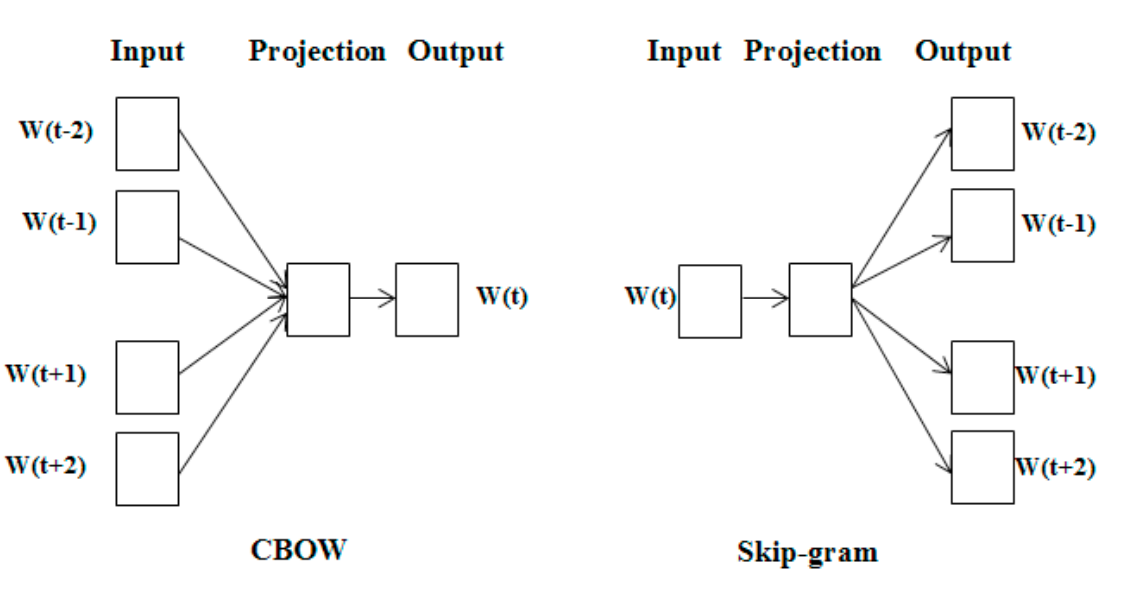
\includegraphics[width=0.5\linewidth]{figures/skip_gram_vs_cbow.png}
    \caption{CBOW vs Skip-gram word embedding models, \cite{jatnika_word2vec_2019}}
    \label{fig:enter-label}
\end{figure}

When using word embeddings in recurrent neural networks, it is usual to include what is called an embedding layer as the first layer of the network. The function of this layer is to train and tailor the word embeddings to better suit the specific task of the network. The reason I say tailor is because the amount of needed data and computational power to create and train word embedding set for a dictionary of any substantial size is quite large it is normal to use pre-trained word embedding datasets and fine-tune these through the embedding layer to better suit the task of the specific network. As we were not sure as to what our task for the network would be specifically we decided a static pre-trained word embedding dataset would suffice, meaning we decided to omit the embedding layer and not train the embedding in the dataset any further to fine-tune them for our network. This will probably limit our results a bit, however, given we don't have any specific categories or themes in mind for our training data the, general word embeddings should suffice.
To take care of the translation to and from the vector space, and find the cosine similarity between word embeddings, we are using the \cite{ines_montani_explosionspacy_2023} python library, which also provides us with a selection of pre-trained word embedding datasets. These datasets range from the smallest containing 50-dimensional word embeddings to the biggest containing 300-dimensional word embeddings.

\section{Results}

When it comes to results the network won't be breaking any records, however, it does perform at a level where we can say it does what it is supposed to, both for predicting sequential numeric data such as a sine wave and for textual data converted to either one-hot encodings or word embeddings, which was the main goal for this model. For the sine prediction, we asked the model to predict the next point of data given a random start value and then passed the result from the prediction back into the model to predict the next value again. We did this after training the model on several sine waves with different noise levels added. Here is the result from predicting the sine:

Loss:
\begin{figure}
    \centering
    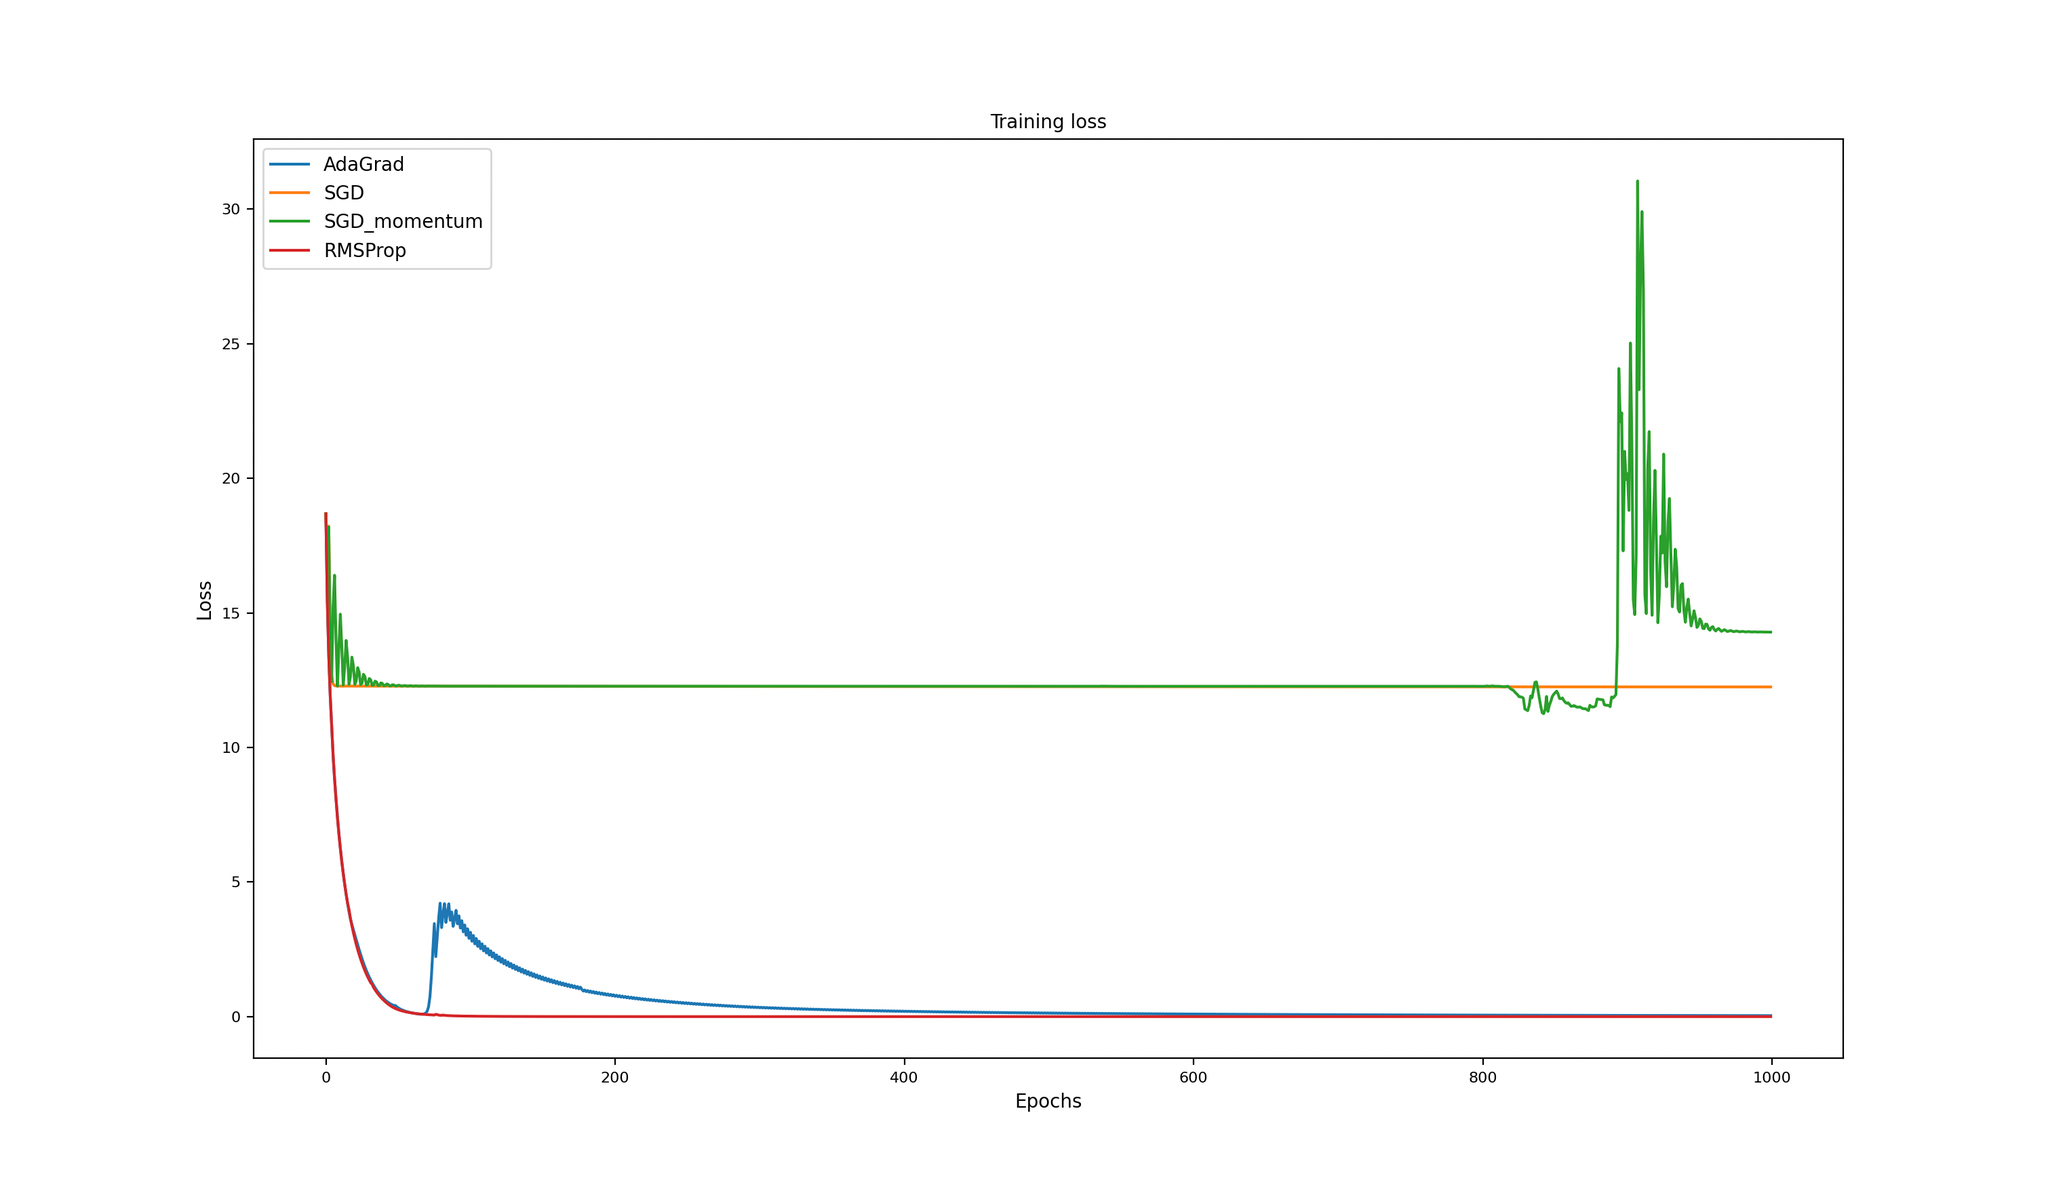
\includegraphics[width = \textwidth]{texfiles/images/dummy_loss.png}
    \caption{DUMMY LOSS, NOT ACTUAL RESULT}
    \label{fig:enter-label}
\end{figure}

Sine:
\begin{figure}
    \centering
    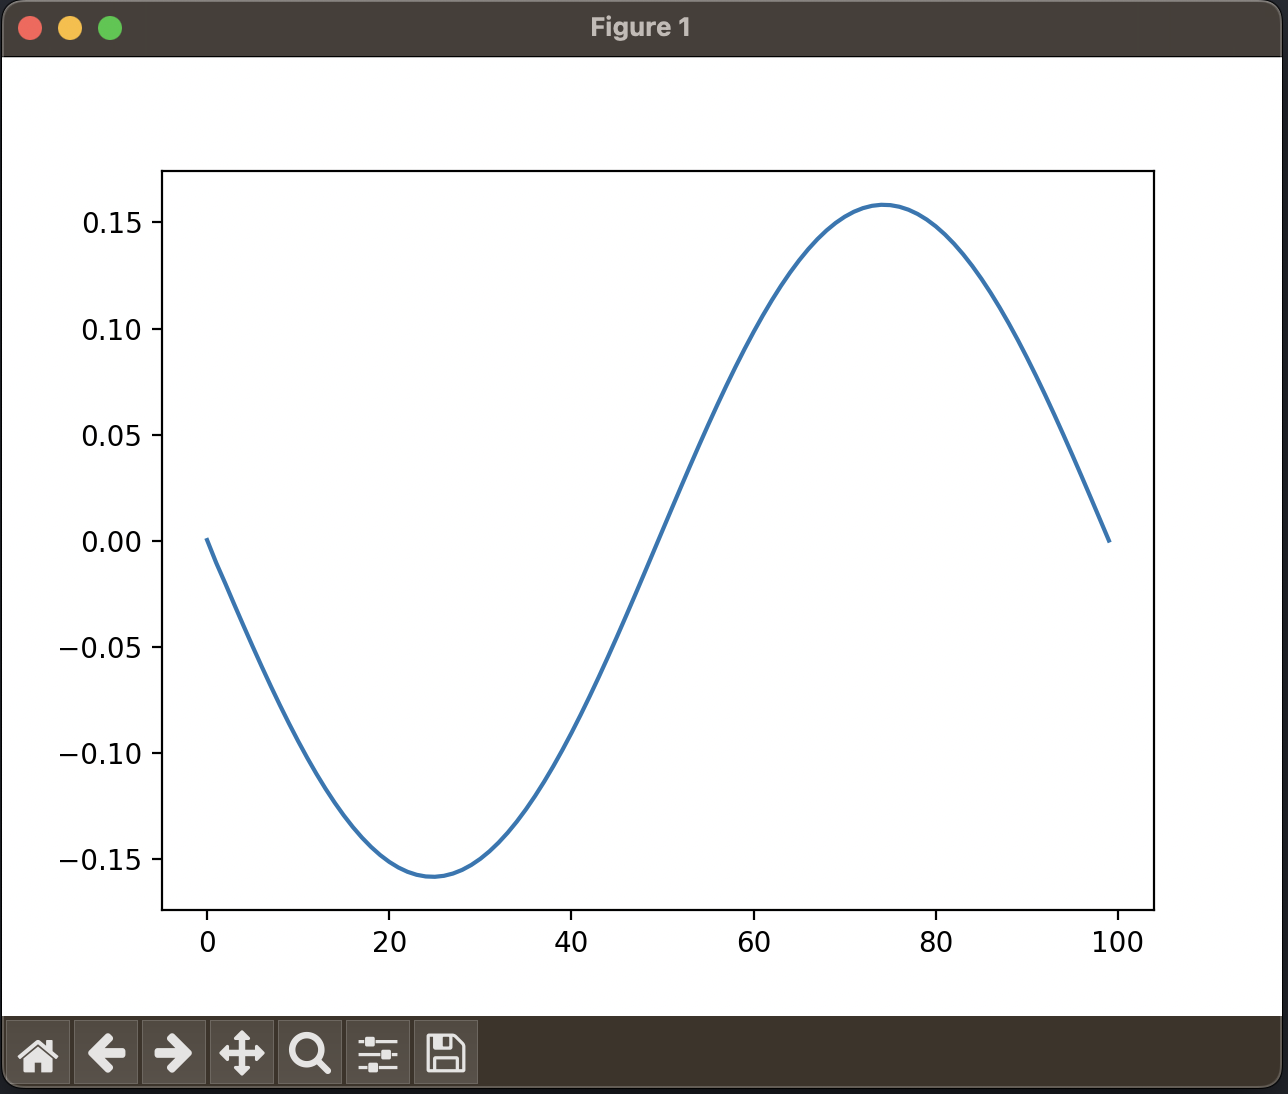
\includegraphics[width = \textwidth]{texfiles/images/sine.png}
    \caption{DUMMY SINE, NOT ACTUAL RESULT}
    \label{fig:enter-label}
\end{figure}

When predicting the next n specified words given a start word to the model, the model presented the following results: 

Loss:
\begin{figure}
    \centering
    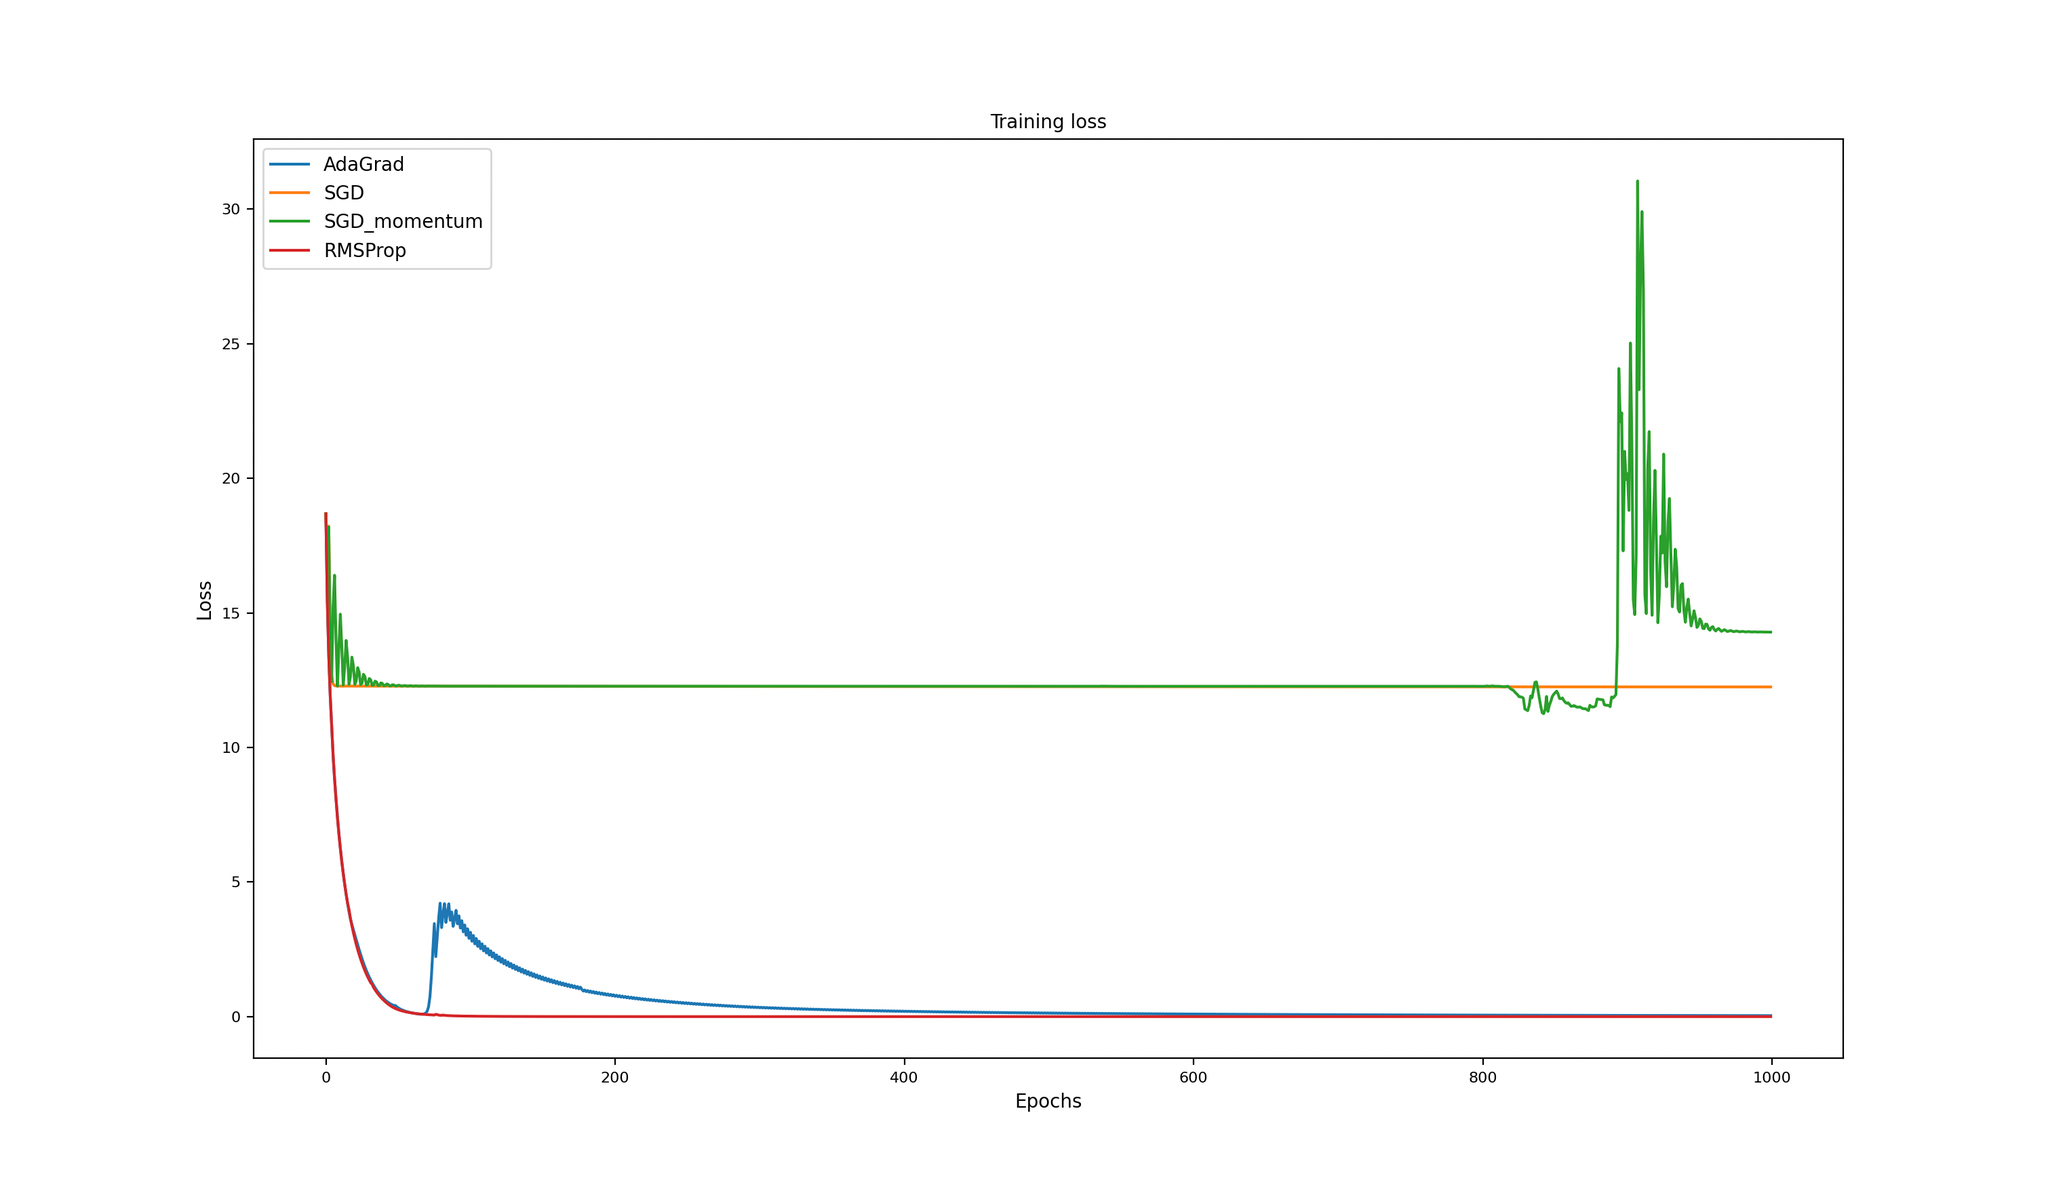
\includegraphics[width = \textwidth]{texfiles/images/dummy_loss.png}
    \caption{DUMMY LOSS, NOT ACTUAL RESULT}
    \label{fig:enter-label}
\end{figure}

Words:
\begin{figure}
    \centering
    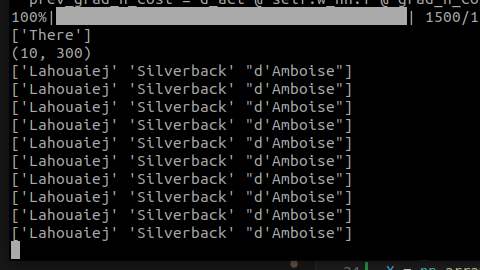
\includegraphics[width = \textwidth]{texfiles/images/dummy_words.png}
    \caption{DUMMY WORDS, NOT ACTUAL RESULT}
    \label{fig:enter-label}
\end{figure}

For one-hot encoding predicting the n specified next characters when passing an initial start character to the model, these were the results: 

Loss:
\begin{figure}
    \centering
    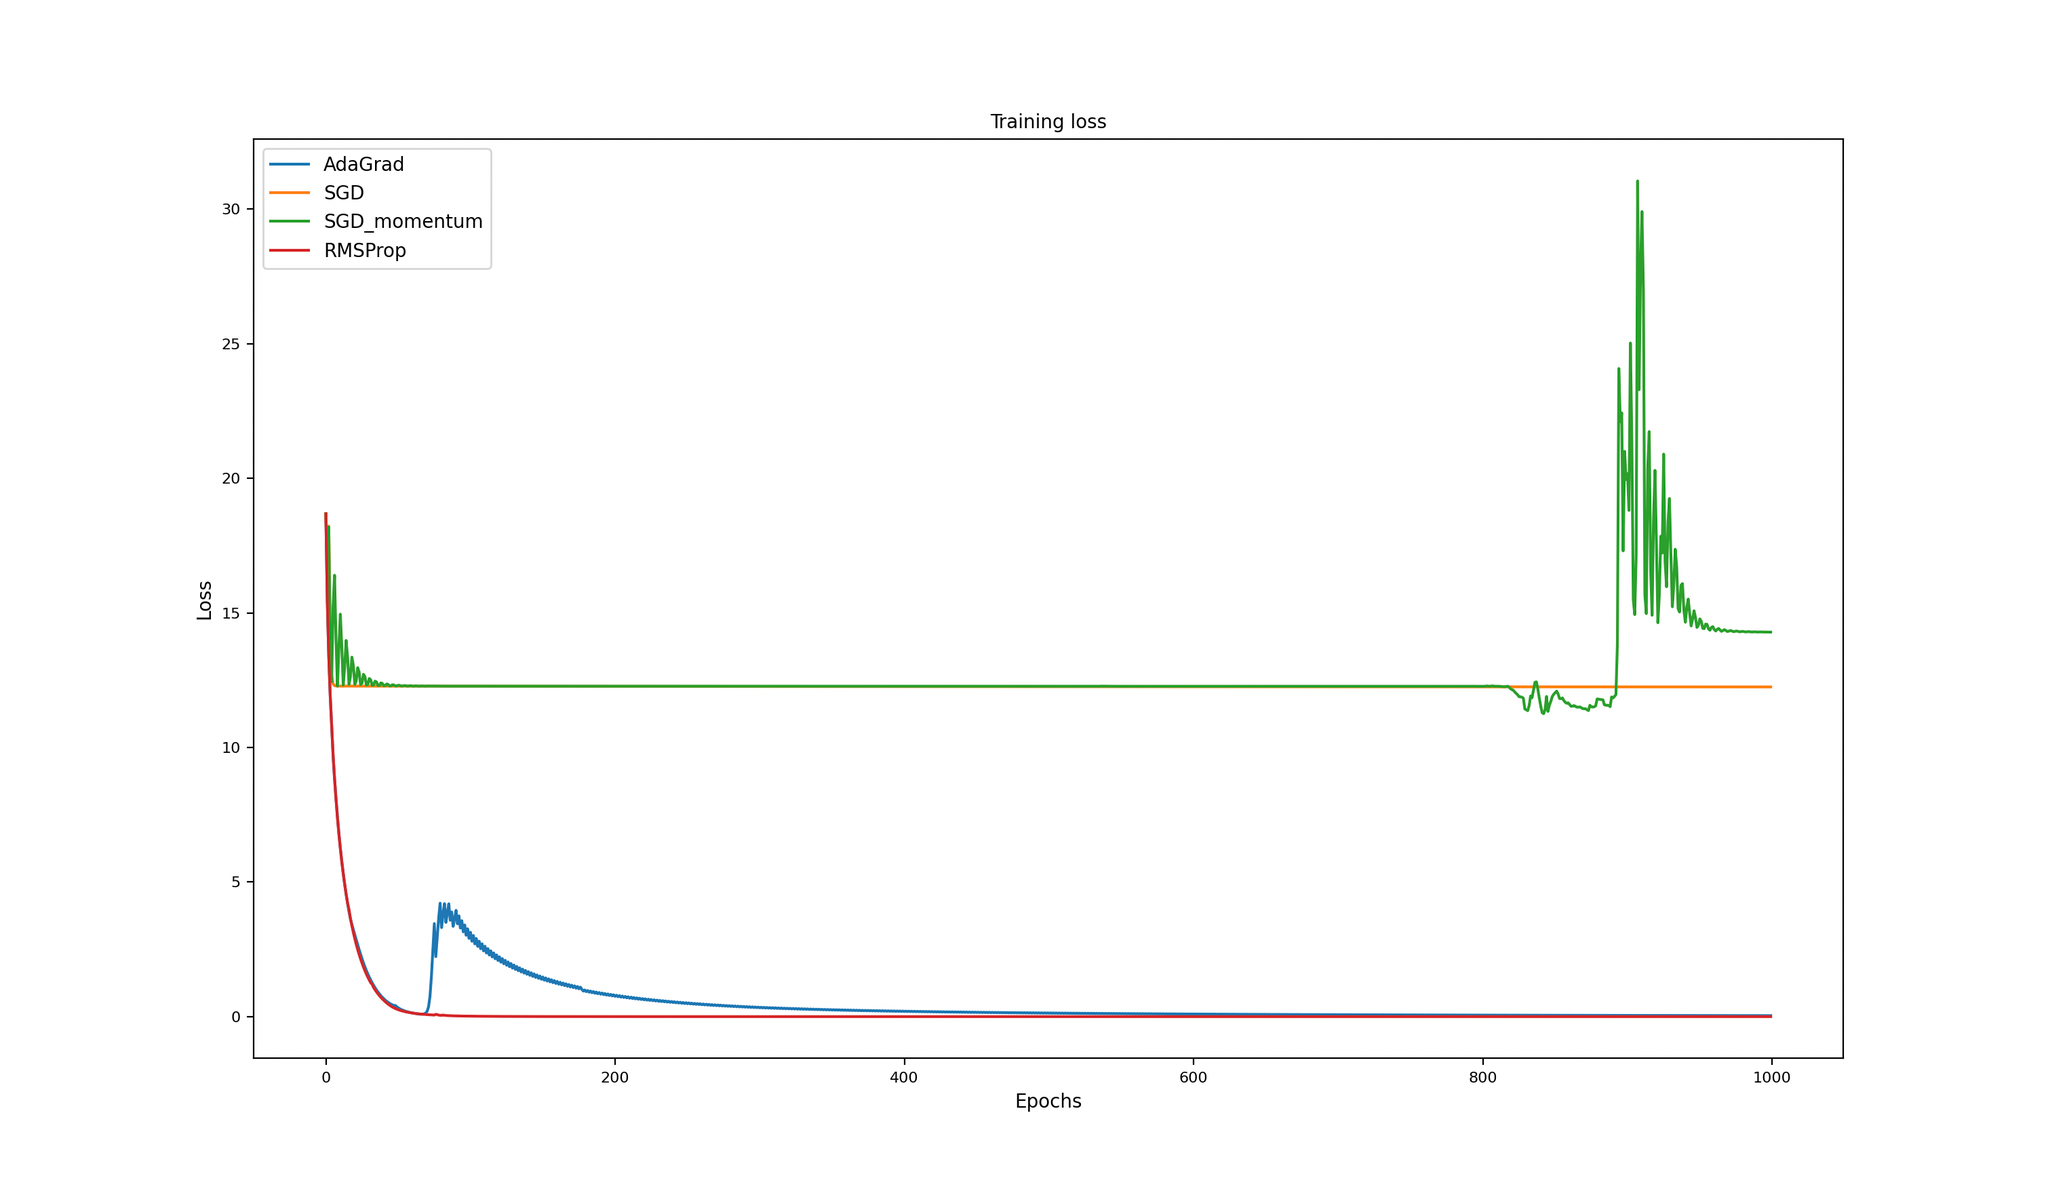
\includegraphics[width = \textwidth]{texfiles/images/dummy_loss.png}
    \caption{DUMMY LOSS, NOT ACTUAL RESULT}
    \label{fig:enter-label}
\end{figure}

Characters:
\begin{figure}
    \centering
    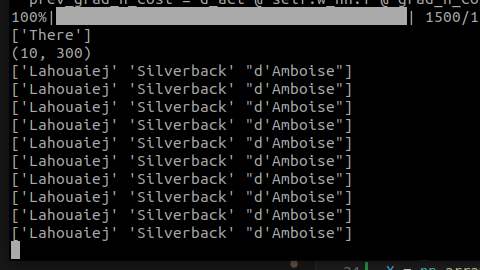
\includegraphics[width = \textwidth]{texfiles/images/dummy_words.png}
    \caption{DUMMY WORDS, NOT ACTUAL RESULT}
    \label{fig:enter-label}
\end{figure}

\section*{Appendix - some math notes}



\printbibliography


\end{document}